\documentclass{llncs}
\usepackage{graphicx, subfigure, amsmath, xspace, txfonts}

\begin{document}
\newcommand{\comment}[1]{}

\author{Jan David Mol, John W. Romein and Rob V. van Nieuwpoort}
\title{The LOFAR Beam Former: \\ Implementation and Performance Analysis}
\institute{Stichting ASTRON (Netherlands Institute for Radio Astronomy) \\ Oude Hoogeveensedijk 4, 7991 PD Dwingeloo, The Netherlands \\ \texttt{\{mol,romein,nieuwpoort\}@astron.nl}}
\maketitle


\begin{abstract}
Radio telescopes typically use large steel dishes to point at and observe radio sources. The LOFAR radio telescope is different, and uses tens of thousands of fixed antennas instead, a novel design which allows many ground-breaking features for radio astronomy. One such a feature is the fact that LOFAR observes omnidirectionally, and focusses by accumulating the signals of its antennas in software in real time. In fact, the parallel processing power and high-speed interconnect in our supercomputer allows us to look at hundreds of sources at the same time. The power to observe many sources in parallel serves a broad range of scientific astronomical interests, and creates novel opportunities for performing astronomical observations.

LOFAR is also the first major telescope to process its data in software, instead of needing a dedicated hardware design. By using software, the processing remains flexible and scalable, and new features are easier to implement and to maintain. It is through the use of software that we can fully explore the novel features and the power of our unique instrument.

In this paper, we present the processing pipeline in our supercomputer which enables our parallel observations. Our so-called \emph{Pulsar Pipeline} is implemented on a supercomputer, and receives up to 64 data streams from the stations at 3.1 Gb/s each. Inside the supercomputer, signal-processing techniques, weighted addition, and two all-to-all exchanges are performed. Our pulsar pipeline further expresses the power of a software telescope implemented using parallel processing techniques. We present the trade-offs in our design, the CPU and I/O performance bottlenecks that we encounter, as well as the scaling characteristics and its real-time behaviour. 
      
\comment{
  
}
\end{abstract}
\section{Introduction}

\comment{
  EUROPAR 2011:
    - abstract 24 jan
    - deadline 31 jan
    - 12 pagina's LNCS, incl broncode
}

\comment{
lofar:
  - overview
  - #stations
  - data rates

pulsar pipeline:  
  - new astronomical opportunities:
        - dynamic focus -> hundreds of simultaenous observations, which regular dishes must do sequentially
        - broad sky view -> surveys
        - extremely high data rates (up to 200 Gbit/s in, 18 Gbit/s out)
                - disks limits output rate, to be raised to 80Gbit/s out.

==> power of parallel machines + flexibility of software = powerful telescope                

software correlator benefits:
  the- flexibility
  - fast rollout of experimental features
  - easy bugfixing
  - high level programming -> advanced and complex features

}

The LOFAR (LOw Frequency ARray) telescope is the first of a new generation of radio telescopes. Instead of using a set of large, expensive dishes, LOFAR uses many thousands of simple antennas. Every antenna observes the full sky, and the telescope can be aimed through signal processing techniques. LOFAR's novel design allows the telescope to perform wide-angle observations as well as to observe in multiple directions simultaneously, neither of which are possible when using traditional dishes. In several ways, LOFAR will be the largest telescope in the world, and will enable ground-breaking research in several areas of astronomy and particle physics~\cite{Bruyn:02}.

Another novelty is the elaborate use of software to process the telescope data in real time. Previous generations of telescopes depended on custom-made hardware to combine data, because of the high data rates and processing requirements. The availability of sufficiently powerful supercomputers however, allow the use of software to combine telescope data, creating a more flexible and reconfigurable instrument.

For processing LOFAR data, we use an IBM BlueGene/P (BG/P) supercomputer. The LOFAR antennas are grouped into stations, and each station sends its data (up to 198 Gb/s for all stations) to the BG/P super computer. Inside the BG/P, the data are split and recombined using both real-time signal processing routines as well as two all-to-all exchanges. The output data streams are sufficiently reduced in size in order to be able to stream them out of the BG/P and store them on disks in our storage cluster.

The stations can be configured to observe in several directions in parallel, but have to divide their output bandwidth among them. In this paper, we present the \emph{beamformer}, an extension to the LOFAR software which allows the telescope to be aimed in tens of directions simultaneously at LOFAR's full observational bandwidth, and in hundreds of directions at reduced bandwidth. Both feats cannot be matched by any other telescope. The data streams corresponding to each observational direction, called \emph{beams}, are generated through (weighted) summations of the station inputs, which are demultiplexed using an all-to-all exchange, and routed to the storage cluster.

The primary scientific use case driving the work presented in this paper is pulsar research. A pulsar is a rapidly rotating, highly magnetised neutron star, which emits electromagnetic radiation from its poles. Similar to the behaviour of a lighthouse, the radiation is visible to us only if one of the poles points towards Earth, and subsequently appears to us as a very regular series of pulses, with a period as low as 1.4~ms~\cite{Hessels:06}. Pulsars are relatively weak radio sources, and their individual pulses often do not rise above the background noise that fills our universe. LOFAR is one of the few telescopes which operates in the frequency range (10 -- 240 MHz) in which pulsars are typically at their brightest. Our beamformer also makes LOFAR the only telescope that can observe in hundreds of directions simultaneously with high sensitivity. These aspects make LOFAR an ideal instrument to discover unknown pulsars by doing a sensitive sky survey in a short amount of time, as well as an ideal instrument to study known pulsars in more detail. Astronomers can also use our beamformer to focus on planets, exoplanets, the sun, and other radio objects, with unprecedented sensitivity. Furthermore, our pipeline allows fast broad-sky surveys to discover not only new pulsars but also other radio sources.

In this paper, we will show how a software solution and the use of massive parallellism allows us to achieve this feat. We provide an in-depth study on all performance aspects, real-time behaviour, and scaling characteristics. The paper is organised as follows.

\section{Related Work}

MWA.

LOFAR imaging pipeline \cite{Romein:10a}

\section{LOFAR}
\label{Sec:LOFAR}

The LOFAR telescope consists of many thousands of simple dipole antennas (see Figure \ref{fig:lbafield}), grouped in \emph{stations}. The stations are strategically placed, with 20 stations acting as its center (the \emph{core}) and 24 stations at increasing distances from that core (see Figure \ref{fig:map}). A core station can act as two individual stations in some observational modes. Every station collects and combines the signals from its antennas, and sends the resulting data stream to our IBM BlueGene/P (BG/P) supercomputer at our central processing facility. The BG/P combines the data streams from one or more stations and reduces the resulting stream in size sufficiently to be able to store it on disks in our storage cluster. Both the stations and the BG/P perform hard-real-time signal processing. Once the data has been stored on disk, off-line processing takes over. The off-line processing transforms and further reduces the data produced by the BG/P into data products such as images or time series, and are made available to the astronomer(s) that requested the observation.

\begin{figure}[ht]
\subfigure[A field with low-band antennas (dipoles).]{
  \makebox[35mm][c]{
     \includegraphics[width=0.3\textwidth]{LBA-field.jpg}
     \label{fig:lbafield}
  }
}
\hfill
\subfigure[Locations of the stations.]{
  \makebox[40mm][c]{
     \includegraphics[width=0.35\textwidth]{lofar-stations.pdf}
     \label{fig:map}
  }
}
\hfill
\subfigure[The left antenna receives the wave later.]{
  \makebox[30mm][c]{
    \includegraphics[width=0.25\textwidth]{delay.pdf}
    \label{fig:delay}
  }
}
\caption{LOFAR antennas}
\end{figure}

The antennas are omnidirectional and have no moving parts. Instead, all telescope functions are performed electronically through signal processing done at the stations and on the BG/P. The telescope can be aimed because the speed of light is finite: the light emitted by a source will arrive at different antennas at different times (see Figure \ref{fig:delay}). By adding appropriate delays to the signals from individual antennas before accumulating them, the signals from the source will be amplified with respect to signals from other directions. Once the samples from all antennas are combined, the data are transmitted to the BG/P, which uses the same technique to combine the data from the individual stations. The latter will be explained further in Section \ref{Sec:Beamforming}.

A LOFAR station is able to produce 248 frequency subbands of 195~kHz out of the sensitivity range of 80~MHz to 250~MHz. Each sample consists of two complex 16-bit integers, representing the amplitude and phase of the X and Y polarizations of the antennas. The resulting data stream from a station is a 3.1~Gb/s UDP stream.

\comment{
  Hardware:
    - stations and antennas
    - network

  Processing in general:
    - station processing
        - how aiming works
    - online processing
    - offline processing
}

\section{IBM BlueGene/P}

We use an IBM BlueGene/P (BG/P) supercomputer for the real-time processing of station data. We will describe the key features of the BG/P, but more information can be found elsewhere~\cite{IBM:08}. Furthermore, we will describe how our BG/P is connected to its input and output systems.

\subsection{System Description}

Our system consists of 3 racks, with 12,480 processor cores that provide 42.4 TFLOPS peak processing power. One chip contains four PowerPC~450 cores, running at a modest 850~Mhz clock speed to reduce power consumption and to increase package density. Each core has two floating-point units (FPUs) that provide support for operations on complex numbers. The chips are organised in \emph{psets}, each of which consists of 64 cores for computation (\emph{compute cores}) and one chip for communication (\emph{I/O node}). Each compute core runs a fast, simple, single-process kernel (the Compute Node Kernel, or CNK), and has access to 512 MiB of memory. The I/O nodes consist of the same hardware as the compute nodes, but additionally have a 10~Gb/s Ethernet interface connected. Also, they run Linux, which allows the I/O nodes to do full multitasking. One rack contains 64 psets, which is equal to 4096 compute cores and 64 I/O nodes.

The BG/P contains several networks. A fast \emph{3-dimensional torus\/} connects all compute nodes and is used for point-to-point and all-to-all communications. The torus uses DMA to offload the CPUs and allows asynchronous communication. The \emph{collective network\/} is used for MPI collective operations, but also for external communication. External communication is routed within each pset, through its I/O node using a tree configuration. The I/O node is capable of transporting 6.8~Gb/s bidirectionally to and from one or more compute nodes. In both networks, data is routed through compute nodes using a shortest path. Additional networks exist for fast barriers, initialization, diagnostics, and debugging. % TODO: add cross-section/link bandwidth for 3D torus?

\subsection{External Networks}
\label{Sec:Networks}

\begin{figure}[ht]
\begin{minipage}[t]{0.47\textwidth}
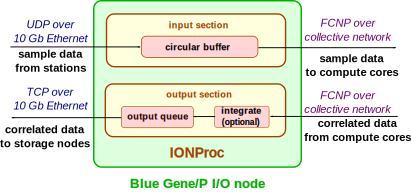
\includegraphics[width=\textwidth]{ION-processing.pdf}
\caption{Data flow diagram for the I/O nodes.}
\label{fig:ion-processing}
\end{minipage}
\hfill
\begin{minipage}[t]{0.3\textwidth}
\center
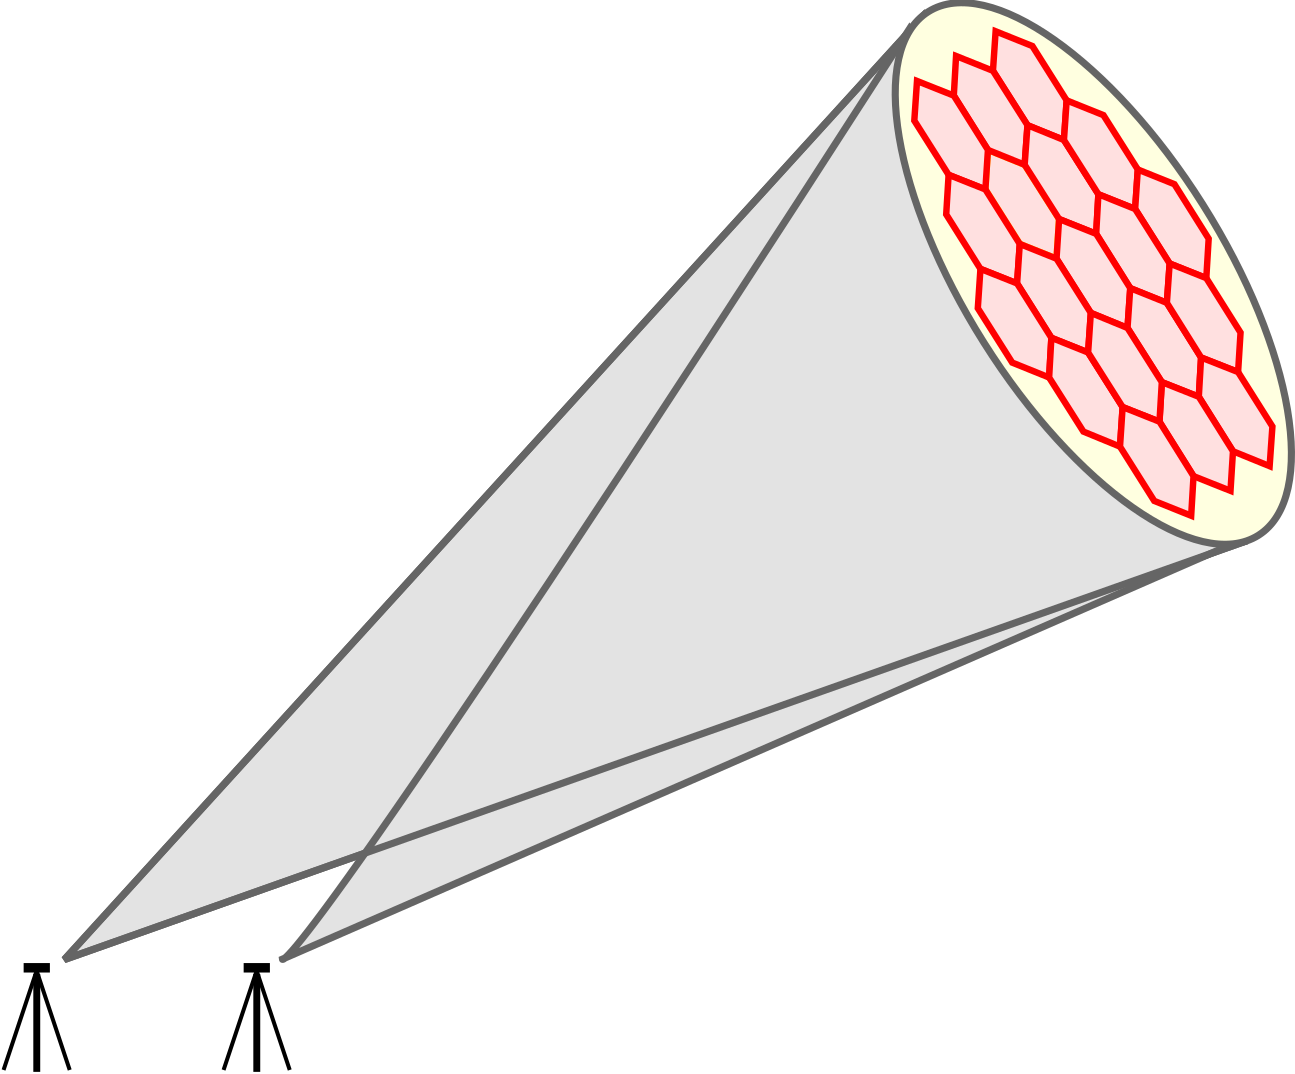
\includegraphics[width=0.8\textwidth]{pencilbeams.pdf}
\caption{Tied-array beams (hexagons) formed within a station beam (ellipse).}
\label{fig:pencilbeams}
\end{minipage}
\end{figure}


We run a multi-threaded program on each I/O~node which is responsible for two tasks: the handling of input, and the handling of output (see Figure \ref{fig:ion-processing}). Even though the I/O nodes each have a 10~Gb/s Ethernet interface, they do not have enough computation power to handle 10~Gb/s of data. The overhead of handling IRQs, IP, and UDP/TCP put such a high load on the 850~MHz cores of the I/O nodes, that the performance seems limited to a total data rate of roughly 4~Gb/s. To achieve these data rates, we installed our own software on the I/O nodes, augmenting IBM's software stack~\cite{Yoshii:10}, and we implemented a low-overhead communication protocol called FCNP~\cite{Romein:09a} to efficiently transport data to and from the compute nodes. Recall that at full observational bandwidth, a station produces 3.1~Gb/s of data. Each I/O node can thus receive data from at most one station. The I/O nodes forward the station data to the compute nodes. The compute nodes convert the (complex) integer samples to the (complex) float domain, and perform all of the necessary on-line signal processing.

Once the compute nodes have finished processing the data, the results are sent back to the I/O nodes. The I/O nodes forward these results to our 24-node storage cluster. Each I/O node can send up to 1.1~Gb/s if it receives station data at the same time, and up to 3.1~Gb/s if the I/O node is not receiving station data. The storage cluster itself can handle up to 80~Gb/s of sustained throughput. The output queue which is maintained at the I/O node for all data uses a best-effort policy and drops data if it cannot be sent, in order to keep the BG/P running at real time.

\comment{
  BG/P explanation:
    - basic architecture and size of our installation
    - IO nodes and compute nodes
    - internal networks
    - external networks and storage nodes
}

\section{Beamforming}
\label{Sec:Beamforming}

As mentioned in Section \ref{Sec:LOFAR}, a LOFAR station is aimed at a source by applying different delays to the signals from the antennas, and subsequently adding the delayed signals. Delaying the signals is known as \emph{delay compensation}, and subsequently adding them as \emph{beamforming}, which is performed at several stages in our processing pipeline. The station beamformer is implemented in hardware, in which the signal is delayed by switching it over wires of different lengths. The signals from the different antennas are subsequently added using an FPGA. The resulting \emph{station beam}, even though it is aimed at a certain source, is nevertheless still sensitive to signals from a large area around the source. 

The BG/P, in which the signals from all the LOFAR stations come together, again performs delay compensation by adding the appropriate delays to the signals from the various stations, this time in software. Because the beam produced by each station has a large sensitive area around the source, the BG/P beamformer can point at the source at which the station beams are pointing, but also at sources around it. An example is shown in Figure \ref{fig:pencilbeams}. The station beam, represented by an ellipse, is sensitive to a sky region around the source it is pointed at. The BG/P can process the data from the stations such that the focus is shifted to sources within the sensitive region, creating \emph{tied-array beams}, which are represented in the figure by hexagons. The actual width of the station beam, as well as the width of the tied-array beams, depends on the number as well as the locations of the stations used. Hundreds of tied-array beams are typically needed to fully cover the sensitive region of a station beam.

Different tied-array beams are formed by adding the signals from the individual stations over and over again, each time using different delays. The delay that has to be applied depends on the relative positions of the stations and the relative direction of the tied-array beam with respect to the station beam. The delays are applied in software in two phases. First, the streams are aligned by shifting them a whole number of samples with respect to each other, which resolves delay differences up to the granularity of a single sample. Then, the remaining sub-sample delays are compensated for by shifting the phase of the signal. Even though a phase correction is not a proper shift because information does not shift between one sample and the next, the difference proves to be sufficiently small in practice.

This approximation is in fact good enough to limit the generation of different tied-array beams through phase corrections alone. The samples coming from different stations are shifted the same amount for all beams that are created. Because a phase shift can be performed using a complex multiplication, the beam former in the BG/P only has to accumulate the weighted vectors of samples from each station. Let $\overrightarrow{S_i}$ be the stream of samples from station $i$, $\overrightarrow{B_j}$ the stream of samples of beam $j$, and $w_{ij}$ the phase correction to be applied on station $i$ to represent the required delay for beam $j$. Then, the beam former calculates $\overrightarrow{B_j} = \sum_{i \in \textrm{stations}}w_{ij}\overrightarrow{S_i}$ on the samples of both the X and Y polarisations independently, to obtain beam $j$. The beam former can be easily parallised. As mentioned in Section \ref{Sec:LOFAR}, the station data consist of a sample stream consisting of up to 248 subbands. The subbands are independent and can thus be processed in parallel. Also, the streams can quite trivially be split along the time dimension in order to increase parallelisation. 

A beam $\overrightarrow{B_j}$ formed at the BG/P consists of a stream of complex 32-bit floating point numbers, two for each time sample (representing the X and Y polarisations), which is equal to 6.2~Gb/s at LOFAR's full observational bandwidth. For some observations however, such a precision is not required, and the beams can be reduced in size in order to be able to output more beams in parallel. In this paper, we consider two types of observations. First, we consider \emph{high-resolution} observations, in which an astronomer wants to look at sources at the highest resolution possible. Such observations will typically produce 6.2~Gb/s per beam. The second type of observation is a \emph{many-beams} observations, in which an astronomer wants to survey the sky with as many beams as possible, given a lower bound on the acceptable resolution. Because each individual beam can be recorded with a much lower resolution than in the high-resolution observations, bandwidth becomes available to create more beams.

The two types of observations translate into three modes in which our pipeline can run:
\begin{description}
\item[Complex Voltages] are the untransformed beams as produced by the beamformer. For each beam, the complex 32-bit float samples for the X and Y polarisations are split and stored in two separate files in disk, resulting in two 3.1~Gb/s streams to disk per beam.
\item[Stokes IQUV] parameters represent the polarisation aspects of the signal, and are the result of a domain transformation performed on the complex voltages: $I = X\overline{X} + Y\overline{Y}$, $Q = X\overline{X} - Y\overline{Y}$, $U = 2\mathrm{Re}(X\overline{Y})$, $V = 2\mathrm{Im}(X\overline{Y})$. The transformation is useful for polarisation-related studies. Each Stokes parameter consists of one 32-bit float per time sample, and is stores in a seperate file. The Stokes IQUV mode thus results in four 1.5~Gb/s streams to disk per beam. % TODO: use of Stokes IQUV
\item[Stokes I] represents the power of the signal in the X and Y polarisations combined, and is equal to the Stokes I stream in the Stokes IQUV mode. This mode thus results in one 1.5~Gb/s stream to disk per beam. Integrating the samples over time is supported in this mode. Time integration reduces the bandwidth per beam by an integer factor, but reduces the time resolution as well.
\end{description}

%TODO: Incoherent stokes

%The BG/P is able to produce tens to hundreds of beams, depending on the mode used. As our measurements will show, the Complex Voltages and Stokes IQUV modes will typically hit an I/O bottleneck when transporting the created beams towards the storage cluster. In the Stokes I mode, the bandwidth per beam is lower and can be further reduced using integration. The I/O bottleneck can thus be avoided in Stokes I mode. If the number of beams is increased, an upper limit on the available memory and computational power will be reached instead.

% TODO: incoherent stokes
\section{Pulsar Pipeline}

%To observe known pulsars, our beamformer is put in the high-resolution mode, in which Complex Voltages or Stokes IQUV parameters are recorded at full bandwidth in order to closely study the shapes of the individual pulses.

In this section, we will describe in detail how the full signal-processing pipeline operates, in and around the beamformer. Much of the pipeline's operation and design is similar to our standard imaging pipeline, described in \cite{Romein:10a}.

\subsection{Input from Stations}
The first step in the pipeline is receiving and collecting from the stations on the I/O nodes. Each I/O node receives the data of (at most) one station, and stores the received data in a circular buffer (recall Figure \ref{fig:ion-processing}). If necessary, the read pointer of the circular buffer is shifted a number of samples to reflect the coarse-grain delay compensation that will be necessary to align the streams from different stations, based on the location of the source at which the stations are pointed.

The station data are split into chunks of one subband and approximately 0.25 seconds. Such a chunk is the unit of data on which a compute node will operate. The size of a chunk is chosen such that the compute nodes will have enough memory to perform the necessary operations on them.

To perform beamforming, the compute nodes need chunks from all stations. Unfortunately, an I/O node can only communicate (efficiently) with the compute nodes in its own pset, which makes it impossible to send the chunks directly to the compute cores that will process them. Instead, the I/O node distributes its chunks over its compute cores in a round-robin fashion, after which the compute cores obtain trade different chunks from the same station for the same chunk from different stations, using an all-to-all exchange.

\subsection{First All-to-all Exchange}

The first all-to-all exchange in the pipeline allows the compute cores to distribute the chunks from a single station, and to collect all the chunks of the same frequency band produced by all of the stations. The exchange is performed over the fast 3D-torus network, but with up to 198~Gb/s of station data to be exchanged (=64 stations producing 3.1~Gb/s), special care still has to be taken to avoid network bottlenecks. It is impossible to optimise for short network paths due to the physical distances between the different psets across a BG/P rack. Instead, we optimised the data exchange by creating as many paths as possible between compute cores that have to exchange data. Within each pset, we employ a virtual remapping such that the number of possible routes between communicating cores in different psets is maximised.

The communications in the all-to-all exchange are asynchronous, which allows a compute core to start processing a subband from a station as soon as it arrives, up to the point that data from all stations are required. Communication and computation are thus overlapped as much as possible.

\subsection{Pre-beamforming Signal Processing}

Once a compute core receives a chunk, it can start processing. First, we convert the station data from 16-bit little-endian integers to 32-bit big-endian floating point numbers, in order to be able to do further processing using the powerful dual FPU units present in each core. The data doubles in size, which is the main reason why we implement it \emph{after} the exchange.

Next, the data are filtered by applying a Poly-Phase Filter (PPF) bank, which consists of a Finite Impulse Response (FIR) filter and a Fast-Fourier Transform (FFT). The FFT allows the chunk, which represents a subband of 195~KHz, to be split into narrower subbands (\emph{channels}). A higher frequency resolution allows more precise corrections in the frequency domain, such as the removal of radio interference at very specific frequencies.

Next, fine-grain delay compensation is performed to align the chunks from the different stations to the same source at which the stations are pointed. The fine-grain delay compensation is performed as a phase rotation, which is implemented as one complex multiplication per sample. The exact delays are computed for the begin time and end time of a chunk, and interpolated in frequency and time for each individual sample. %TODO: why a frequency-dependent component?

Next, a band pass correction is applied to adjust the signal strengths in all channels. This is necessary, because the stadions introduce a bias in the signal strengths across the channels within a subband.

Up to this point, processing chunks from different stations can be done independently, but from here on, the data from all stations are required. The first all-to-all exchange thus ends here.

\subsection{Beamforming}

The beamformer creates the beams as described in Section \ref{Sec:Beamforming}. First, the different weights required for the different beams are computed, based on the station positions and the beam directions. Note that the data in the chunks are already delay compensated with respect to the source at which the stations are pointed. Any delay compensation performed by the beamformer is therefore to compensate the delay differences between the desired beams and the station's source. The reason for this two-stage approach is flexibility. By already compensating for the station's source in the previous step, the resulting data can not only be fed to the beamformer, but also to other pipelines, such as the imaging pipeline. Because we have a software pipeline, we can implement and connect different processing pipelines with only a small increase in complexity.

The delays are applied to the station data through complex multiplications and additions. In order to take full advantage of the L1 cache and the available registers, data is processed in sets of 6 stations, producing 3 beams, or a subset thereof to cover the remaining stations and beams. While the exact ideal set size in which the data is to be processed depends on the architecture at hand, we have shown in previous work that similar tradeoffs exist for similar problems across different architectures~\cite{FOO,BAR}.

Because each beam is an accumulated combination of the data from all stations, the bandwidth of each beam is equal to the bandwidth of data from a single station, which is 6.2~Gb/s now that the samples are 32-bit floating point numbers. Once the beams are formed, they can be kept as such (Complex Voltages) or optionally be transformed into the Stokes IQUV or the Stokes I parameters. In the latter case, the beams can also be integrated time-wise, in which groups of samples of fixed size are accumulated together to reduce the resulting data rate.

The beamformer transforms chunks representing station data into chunks representing beam data. Because a chunk representing station data contained data for only one subband, the chunks representing different subbands of the same beam are still spread out over the full BG/P. Chunks corresponding to the same beam are brought together using a second all-to-all exchange.

\subsection{Dedispersion}

TODO

\subsection{Second All-to-all Exchange}

In the second all-to-all exchange, the chunks made by the beamformer are rearranged again using the 3D-torus network. Due to memory constrains on the compute cores, the cores that performed the beamforming cannot be the same cores that receive the beam data after the exchange. Instead, we assign a set of cores (\emph{output cores}) to receive the rearranged chunks of beam data. The output cores are chosen before an observation, and are never scheduled to do participate in the earlier computations in the pipeline (which are done by the \emph{input cores}).

An output core first gathers chunks of beam data that belong to the same beam but represent different subbands. Then, it puts the data in the final ordering, which means both sorting the received chunks and reordering the dimensions of the data within a chunk. Reordering the data within a chunk is necessary, because the data order that will be written to disk is not the same order that can be produced by our computations without taking heavy L1 cache penalties. We hide this reordering cost at the output cores by overlapping computation (the reordering of a chunk) with communication (the arrival of other chunks). Once all of the chunks are received and reordered, they are sent back to the I/O node using the tree network.

For the distribution of the workload over the available output cores, three factors have to be considered. First, all of the data belonging to the same beam has to be processed by output cores in the same pset, in order to ensure that its I/O node can concatenate all of the 0.25 second chunks that belong to the beam. Second, the maximal output rate of the I/O node has to be considered. As mentioned in Section \ref{Sec:Networks}, an I/O node can output 1.1~Gb/s if it is processing station input data, and 3.1~Gb/s if it is not. However, a complex-voltages beam is 6.2~Gb/s. We therefor optionally split each beam into two or more substreams, each of which will be output by a separate I/O node and each of which will eventually end up as a seperate file on disk. For example, we store the X and Y polarisation data of a complex-voltages beam in two separate files. If there are not enough I/O nodes which do not process station input data, the X and Y polarisations have to be split further, in which case we store 82 or 83 subbands per file, with 3 files per polarisation.

A third factor in the scheduling of the output cores is the presence of the first all-to-all-exchange, which uses the same network at up to 198~Gb/s. The second exchange uses up to 80~Gb/s. Careful planning of the workload distribution is necessary, because the 3D-torus network routes data over other compute nodes, with each link sustaining 3.4~Gb/s. Some network links in the BG/P become overloaded unless enough output cores are used to spread the load.

\subsection{Transport to Disks}
Once an output core has received and reordered all of its data, the data are sent to the core's I/O node. The I/O node forwards the data over TCP/IP to the storage cluster. To avoid any stalling in our pipeline due to network congestion or disk issues, the I/O node uses a best-effort buffer which drops data if it cannot be sent.

\comment{
  Pulsar pipeline (include picture):
     - 1st transpose
     - pre-beamforming signal processing 
     - beam forming / stokes
     - pre-transpose reordering
     - 2nd transpose
     - post-transpose reordering
     - send to storage

  Notable comments:
     - optimal split of 6 stations, 3 beams, 128 samples for beam former, due to L1 cache and #registers.
       is a more general problem, see ppopp and ics papers.
     - software allows fast roll-out and testing of features, flexible flow control, and only
       optimisation where needed but maintainability elsewhere.
}

\section{Performance Analysis}

We will focus our performance analysis on edge cases that are of astronomical interest. In all cases, we respect the real-time nature of our system by limiting the load such that there is at most 0.1\% of data loss. Almost all variance occurs in the networks within the BG/P due to clashes caused by scheduling intricacies.

\subsection{Overall Performance}

% TODO: getallen kloppen niet.. 13 beams is 80.6 Gb/s, en met 70 Gb/s zouden we 11 beams aan moeten kunnen
Figure \ref{fig:stations-beams} shows the maximum number of beams that can be created when using a various number of stations, in each of the three modes: Complex Voltages, Stokes IQUV, and Stokes I. In both the Complex Voltages and the Stokes IQUV modes, the pipeline is I/O bound. Each beam is 6.2~Gb/s wide. We can make at most 12 beams without exceeding the available 80~Gb/s to our storage cluster. The available bandwidth decreases down to 70~Gb/s due to the fact that an I/O node can only output 1.1~Gb/s if it also has to process station data. The granularity with which the output can be distributed over the I/O nodes, as well as scheduling details, determine the actual number of beams that can be created, but in all cases, the beamformer can create at least 10 beams at LOFAR's full observational bandwidth.

In the Stokes I mode, we applied several integration factors (1, 2, 4, 8, and 12) in order to show the trade-off between beam quality and the number of beams. Integration factors higher than 12 does not allow significantly more beams to be created, but could be used in order to further reduce the total output rate. For low integration factors, the beam former is again limited by the available output bandwidth. Once the Stokes I streams are integrated sufficiently, the system becomes bounded by the compute nodes: if only signals from a few stations have to be combined, the beam former is limited by the amount of available memory required to store the beams. If more input has to be combined, the beam former becomes limited by the CPU power available in the compute cores. For observations for which a high integration factor is acceptable, the beam former is able to create 155 up to 543 tied-array beams, depending on the number of stations used. For observations which need a high time resolution and thus a low integration factor, the beam former is still able to create at least 42 tied-array beams.

\subsection{System Load}

\begin{table}
\begin{tabular}{l|l|r|r|r|r|r|r|l|l}
Case & Mode & Coherent     & Integration & Stations & Beams  & Input & Output & Bound & Used for \\
     &      & dedispersion & factor      &          &        & rate  & rate   &       & \\
\hline
\hline
A & Stokes I    & N & 12 &  4 & 543 &  12 Gb/s & 70 Gb/s & Memory & Surveys \\
B & Stokes I    & N &  8 & 24 & 327 &  74 Gb/s & 63 Gb/s & CPU   & Surveys \\
C & Stokes I    & N &  8 & 64 & 155 & 198 Gb/s & 30 Gb/s & CPU   & Surveys \\  
D & Stokes IQUV & Y & - & 24 &  13 &  74 Gb/s & 80 Gb/s & I/O   & Known sources \\
E & Stokes IQUV & Y & - & 64 &  10 & 198 Gb/s & 62 Gb/s & I/O   & Known sources \\
F & Stokes I    & Y & 1 & 64 &  42 & 198 Gb/s & 65 Gb/s & CPU   & Known sources 
\end{tabular}
\caption{Several highlighted cases.}
\label{table:cases}
\end{table}

We further analyse the workload of the compute cores by highlighting a set of interesting cases, summarised in Table \ref{table:cases}. We will focus on a memory-bound case (A), which also creates the highest number of beams, on CPU-bound cases interesting for performing surveys, with either 24 stations (B) or 64 stations (C) as input. Cases D and E focus on high-resolution observations of known sources, and are I/O bound configurations with 24 and 64 stations, respectively. Case F focusses on the observations of known sources as well, using Stokes I output, which allows more beams to be created. Coherent dedispersion requires the DM of the sources to be known, and is thus only enabled in the cases which observe known sources.

The workload of the compute cores for each case is shown in Figure \ref{fig:execution-times}, which shows the average workload per core. For the CPU-bound cases B and C, the average load has to be lower than 100\% in order to prevent fluctuations from slowing down our real-time system. These fluctuations typically occur due to clashes within the BG/P 3D-torus network which is used for both all-to-all-exchanges, and cannot be avoided in all cases.

The cases which create many beams (A-C) spend most of the cycles performing beam forming and calculation the Stokes I parameters. The beamforming scales with both the number of stations and the number of beams, while the Stokes I calculation costs depends solely on the number of beams. Case A has to beam form only four stations, and thus requires most of its time calculating the Stokes I parameters. Case B and C use more stations, and thus need more time to beam form.

The costs for both the first and the second all-to-all exchange are mostly hidden due to overlaps with computation. The remaining cost for the second exchange is proportional to the output bandwidth required in each case.

For the I/O-bound cases D-F, only a few tied-array beams are formed and transformed into Stokes I(QUV) parameters, which produces a lot of data but requires little CPU time. Enough CPU time is therefore avaialable to include coherent dedispersion, which scales with the number of beams and, as Figure \ref{fig:execution-times} shows, is an expensive operation.

\comment{
 - hit CPU, memory and I/O bounds
 - scheduling intricacies
 - <0.1 perc loss
}


\begin{figure}[ht]
\begin{minipage}[t]{0.47\textwidth}
\includegraphics[width=\textwidth]{stations-beams.pdf}
\label{fig:stations-beams}
\caption{The maximum number of beams that can be created in various configurations.}
\end{minipage}
\hfill
\begin{minipage}[t]{0.47\textwidth}
\includegraphics[width=\textwidth]{execution_times.pdf}
\label{fig:execution-times}
\caption{The time spent in the processing steps.}
\end{minipage}
\end{figure}

\comment{
  Intro belooft:
    - performance
    - real-time (relevant in dit paper als performance al onderhanden genomen wordt?)
    - scalability

  Scalability:
    - scale on one rack in #beams

  Performance:
    - percent of peak performance of major components
    - network bw use in 2nd transpose
}

\cite{Hessels:09}

\section{Discussion}

\comment{
  - Lessons learned: a software telescope
  - Astronomical opportunities
}

\section{Conclusions}

\comment{
  We have shown:
    - beam forming implementation to form 200+ beams
    - performance figures
    - results from deployed system
    - power of software telescopes
}

\bibliographystyle{plain}
\bibliography{lofar}

\end{document}
